\documentclass[10pt]{article}
\textheight=9.25in \textwidth=7in \topmargin=-.75in
 \oddsidemargin=-0.25in
\evensidemargin=-0.25in
\usepackage{url}  % The bib file uses this
\usepackage{graphicx} %to import pictures
\usepackage{amsmath, amssymb, bbold}
\usepackage{theorem, multicol, color}
\usepackage{gfsartemisia-euler} % best font in da game
\usepackage{tikz} % Graphs and other graphics

\setlength{\intextsep}{5mm} \setlength{\textfloatsep}{5mm}
\setlength{\floatsep}{5mm}
\setlength{\parindent}{0em} % new paragraphs are not indented
\setcounter{MaxMatrixCols}{20}
\usepackage{caption}
\captionsetup[figure]{font=small}


%%%%  SHORTCUT COMMANDS  %%%%
\newcommand{\ds}{\displaystyle}
\newcommand{\Z}{\mathbb{Z}}
\newcommand{\1}{\mathbb{1}}
\newcommand{\arc}{\rightarrow}
\newcommand{\R}{\mathbb{R}}
\newcommand{\N}{\mathbb{N}}
\newcommand{\Q}{\mathbb{Q}}
\renewcommand{\P}{\mathbb{P}}
\newcommand{\E}{\mathbb{E}}
\newcommand{\blank}{\underline{\hspace{0.33in}}}
\newcommand{\qand}{\quad and \quad}
\renewcommand{\stirling}[2]{\genfrac{\{}{\}}{0pt}{}{#1}{#2}}
\newcommand{\dydx}{\ds \frac{d y}{d x}}
\newcommand{\ddx}{\ds \frac{d}{d x}}
\newcommand{\dvdx}{\ds \frac{d v}{d x}} 

%%%%  footnote style %%%%

\renewcommand{\thefootnote}{\fnsymbol{footnote}}

\pagestyle{empty}

\begin{document}

\begin{flushright}
Chandler Justice - A02313187
\end{flushright}
\noindent \underline{\hspace{3in}}\\
\textbf{MATH5620:} Homework \#4 \\
\textbf{Due:} March 22, 2024 @ 23:59\\

\textbf{Problem 1:} In this problem you will need to write code to approximately solve the elliptic partial differential equation (PDE). The following PDE is called the Poisson equation. Note that

\[\Delta u = f\]

on $\partial\Omega$, the boundary of the region. This is a region in two spatial dimensions. Write your code to use a domain defined by the unit square. That is, $\Omega = (0,1) \times (0,1)$.\\

Use equally spaced points in the finite different method in both directions as done in class. Choose the same mesh size in both directions. Make sure that the code produced allows the user to use different values of $h$. For the problems below, the code developed for this Question needs to be able to set up the linear system of equations that results from application of the 5-point stencil as discussed in class. we will want to use values of $h$ in the following list.
\[h_i = \left\{\frac{1}{8}, \frac{1}{16}, \frac{1}{32}, \cdots, \frac{1}{2^8}\right\}\]

The code for this Question should handle the setup to the problem up to the choice of linear solver for the linear system of equations that results from the finite difference method.

\textbf{Solution 1:} I wrore the following functions and encapsulated them in a class to complete this portion of the question:

\begin{verbatim}
class poissonSolver:


    def __init__(self, f, n):
        self.h = 1/n
        self.f = f
        self.n = n
        
        # create the interval within the bonudary
        self.x = np.arange(0, 1.00001, self.h)
        self.y = np.arange(0, 1.00001, self.h)


    def build_w(self) -> np.array:
        # build the boundary of the matrix
        # recall g(x,y) = 0
        return np.zeros((self.n**2, self.n**2))


    def build_A(self) -> np.array:
        m = self.n - 1
        A = np.array
        k = [np.ones(m*(m-1)), np.ones((m**2) -1), -4*np.ones(m**2), np.ones((m**2)-1), np.ones(m*(m-1))] 
        offset = [-m,-1,0,1,m]
        A = diags(k, offset).toarray()
        A *= (self.h)**2
        return A


    def build_r(self):
        r = np.zeros((self.n - 1)**2)
        for i in range(0, self.n-1):
            for j in range(0, self.n-1):
                r[i+(self.n-1)*j] = f(i+1, j+1)
        return r


\end{verbatim}

Running this set of functions provides all the setup for solving the linear system of equations\\

\textbf{Problem 2:}A couple of graphcs to see what is going on.\\

Using Matplotlib (or equivalent package) to graph the solutions obtained in the computational convergence study. This means the use a contour plot, a density plot, or a streamline plot. This question needs at least one of the three types of plots above for the question solution to be considered completed. Make sure that your code accepts as input on the two dimensional grid used to define the mesh. You can test this code by graphing the right hand side function in the problem definition. It would pay dividends if the code written for this question could provide a function that you pass the data for the right hand side function at the mesh points and provide plots/graphics of the data. Then you will be able to reuse this code to plot the solutions for the PDE.\\

\textbf{Solution 2:} I wrote the following function to plot the results of my elliptic equation solvers

\begin{verbatim}
def display_solver_convergence():
    r_jacobi = []
    r_numpy = []
    r_conjugate = []

    for i in range(2, 7):
        test = poissonSolver(f, 2**i)
        convergence = test.compute_convergence()
        r_jacobi.append(convergence[0])
        r_numpy.append(convergence[1])
        r_conjugate.append(convergence[2])
    plt.plot(r_jacobi, label= 'jacobi convergence')
    plt.plot(r_numpy, label = 'numpy built-in convergence')
    plt.plot(r_conjugate, label = 'conjugate gradient convergence')
    plt.legend()
    plt.show()
    print(r_jacobi, r_numpy, r_conjugate)
\end{verbatim}

This shows a graph of the rate of convergence for each method (alongside a bonus method I included using all built-in numpy functions).

\textbf{Problem 3:} Build a piece of code or function that implements Jacobi iteration for the linear system that results from the finite difference method used in this assignment. Use a sparse matrix approach that stores only the nonzero entries in the matrix. This means using a vector for each of the diagonals (5) that contain nonzero entries.\\

\textbf{Solution 3:} I wrote the following function to solve the system of equations using Jacobi iteration

\begin{verbatim}
    def solve_system_jacobi(self):
        # use jacobi iteration to solve system of equations
        def jacobi(A, b, N = 25, x=None):
            # Create an initial guess if needed                                                                                                                                                            
            if x is None:
                x = np.zeros(len(A[0]))

            # Create a vector of the diagonal elements of A                                                                                                                                                
            # and subtract them from A                                                                                                                                                                     
            D = np.diag(A)
            R = A - np.diagflat(D)

            # Iterate for N times                                                                                                                                                                          
            for _ in range(N):
                x = (b - np.dot(R,x)) / D
            return x
        A = self.build_A() 
        r = self.build_r()
        return jacobi(A, r)
\end{verbatim}

\textbf{Problem 4:} Repeat the same work as in Question 3. Instead of using the Jacobi Iteration Method, use the Conjugate Gradient method for the solution process. Compare the results on the finest resolution chosen in the list of $h$ values, $h = \frac{1}{2^8}$. Show your results using the graphics code from Question 2. Show graphs of both solution results as part of your write-up.

\textbf{Solution 4:} Here is the function I wrote to compute solutions using the conjugate gradientlinear solution

\begin{verbatim}
    def solve_system_conjugate_gradient(self):
        A = self.build_A()
        r = self.build_r()
        p = r
        x = np.zeros((self.n - 1)**2)
        rsold = np.dot(np.transpose(r), r)
        
        for _ in range(len(r)):
            Ap = np.dot(A, p)
            alpha = rsold / np.dot(np.transpose(p), Ap)
            x = x + np.dot(alpha, p)
            r = r - np.dot(alpha, Ap)
            rsnew = np.dot(np.transpose(r), r)
            if np.sqrt(rsnew) < 1e-8:
                break
            p = r + (rsnew/rsold)*p
            rsold = rsnew
        return x
\end{verbatim}

comparing the computational convergence analysis coeffecients I obtained, we can see \textit{Jacobi Iteration} acheived \verb|1.477090151549603e-23|, while \textit{conjugate gradient method} achieved \verb|5.716707600466546e-24|. Here is the output from my visualization comparing the techniques:

\begin{center}
    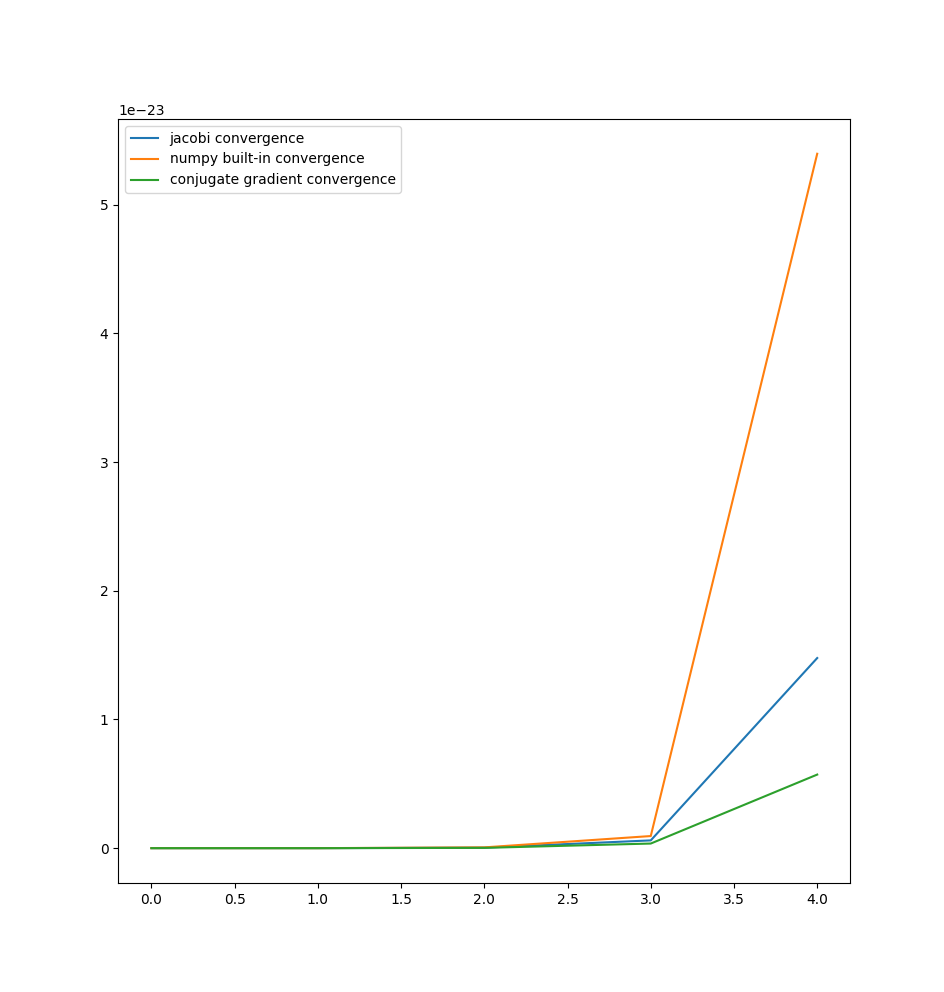
\includegraphics[scale=0.25]{Figure_1.png}
\end{center}
\noindent \underline{\hspace{3in}}\\

\end{document}

